\begin{abstract}
This project attempts to act as a health report for your Hadoop cluster. At its core, this tool acts as a Hadoop
Testing Framework. Tests are either in the form of rules or checks, and either flag the table for review if a rule
fails, or throws a warning if a check fails. Tests can be scheduled, and the incremental output can be viewed through
the local frontend. This allows for the user to view the health and status of their database over time.
\end{abstract}

\section{Introduction}
This tool attempts to perform health checks on your Hadoop cluster through automated scripts that are run. The results
of these scripts can be viewed over time to determine the status of the cluster, and how its status compares to the
last few days.

\section{Checks}
Every test is simply a script that lives in a type-specific folder. Rules and Checks exist separately.

Each script returns a JSON-encoded object to {\ttfamily stdout} that meets the following specification.

\begin{minted}[frame=lines, framesep=2mm, linenos=true]{json}
{
    "name":"Name of test",
    "violations":9000,
    "Output":"Test Specific output. Either JSON or String"
}
\end{minted}


    \subsection{Rules}
    Rules are strict rules about the cluster. They should never be ignored, or disobeyed, and any violation of a set rule
    results in a violation. Ideally, a ``healthy'' cluster should have no rule violations.

    An example rule would be that a specific column only contains integers.

    \subsection{Warning}
    Checks are suggestions about specific tables, or databases. These are a lot more fluid, and a warning from a check does
    not necessarily indicate an issue with the database, but rather that something new may have happened.

    For example, a check that examines the average number of a column may throw a warning if an entry is too far from the
    mean. This isn't an indication that the data is bad, just that it \textit{may} be bad.

\section{Results}
All results can be viewed through the front end. This provides a way to analyze your cluster's health, as well as its
current status.

\begin{figure}[H]
    \centering
    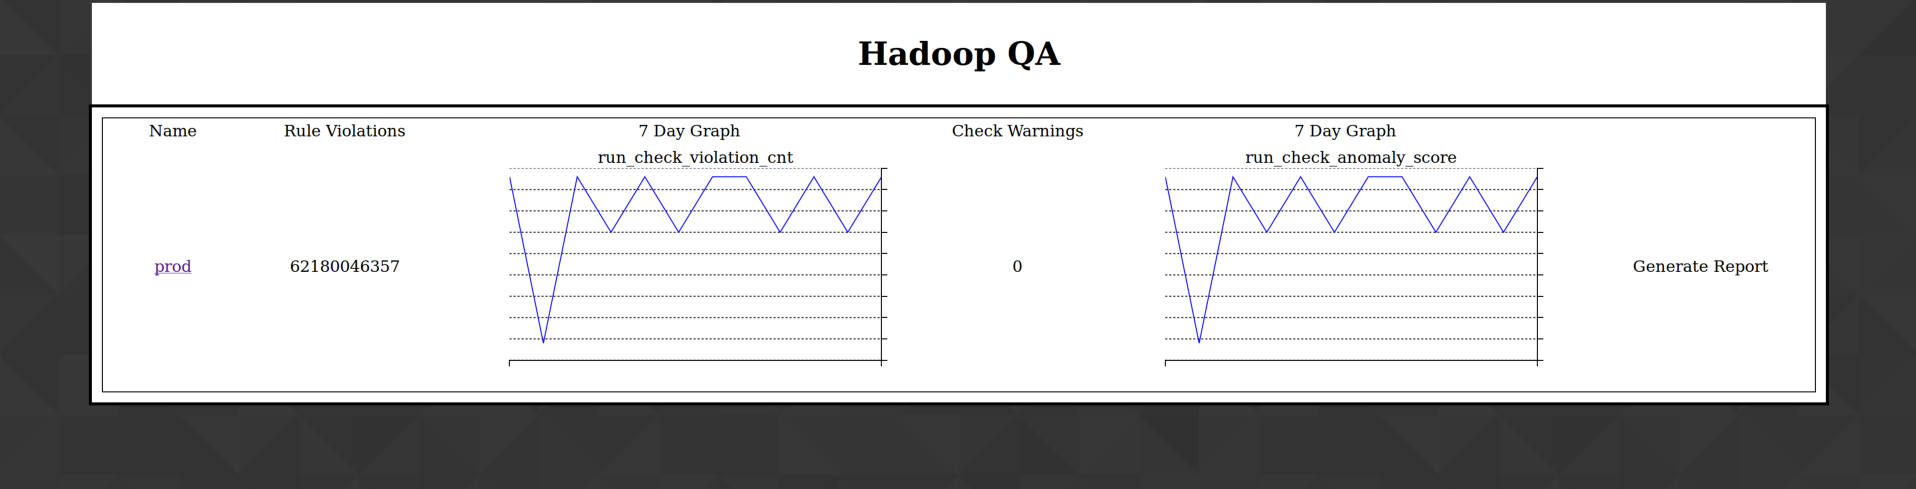
\includegraphics[scale=0.2]{./img/index.png}
    \caption{Index}
\end{figure}

\begin{figure}[H]
    \centering
    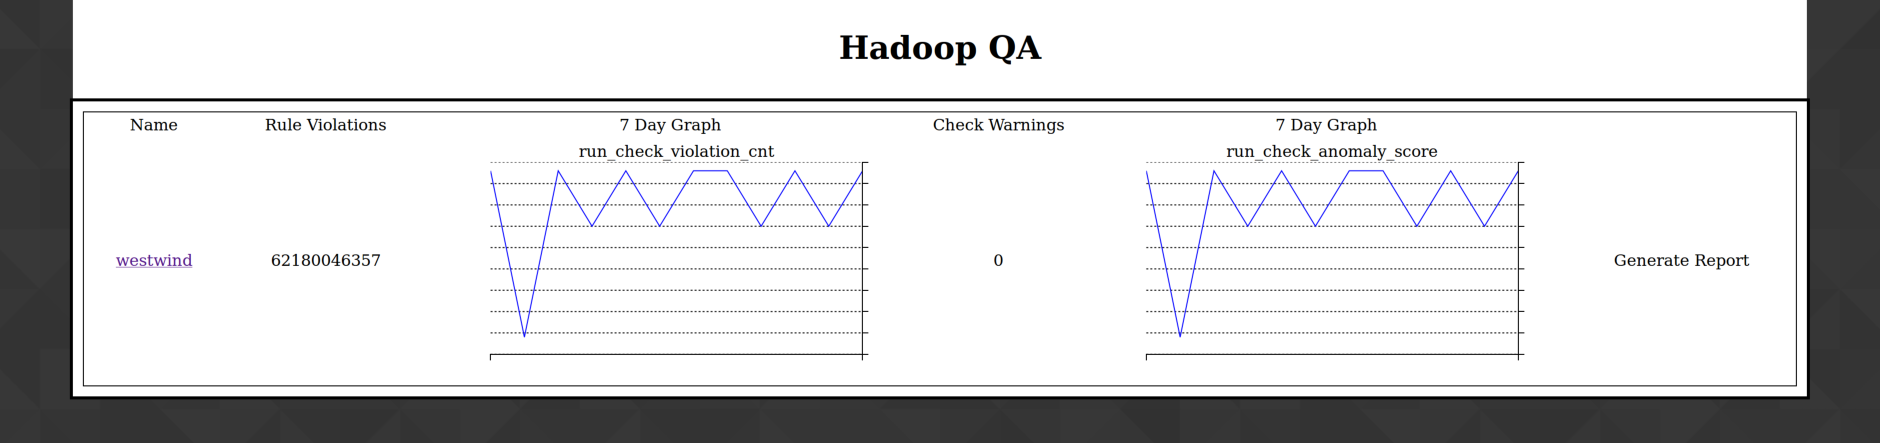
\includegraphics[scale=0.2]{./img/prod.png}
    \caption{Environment View}
\end{figure}

\begin{figure}[H]
    \centering
    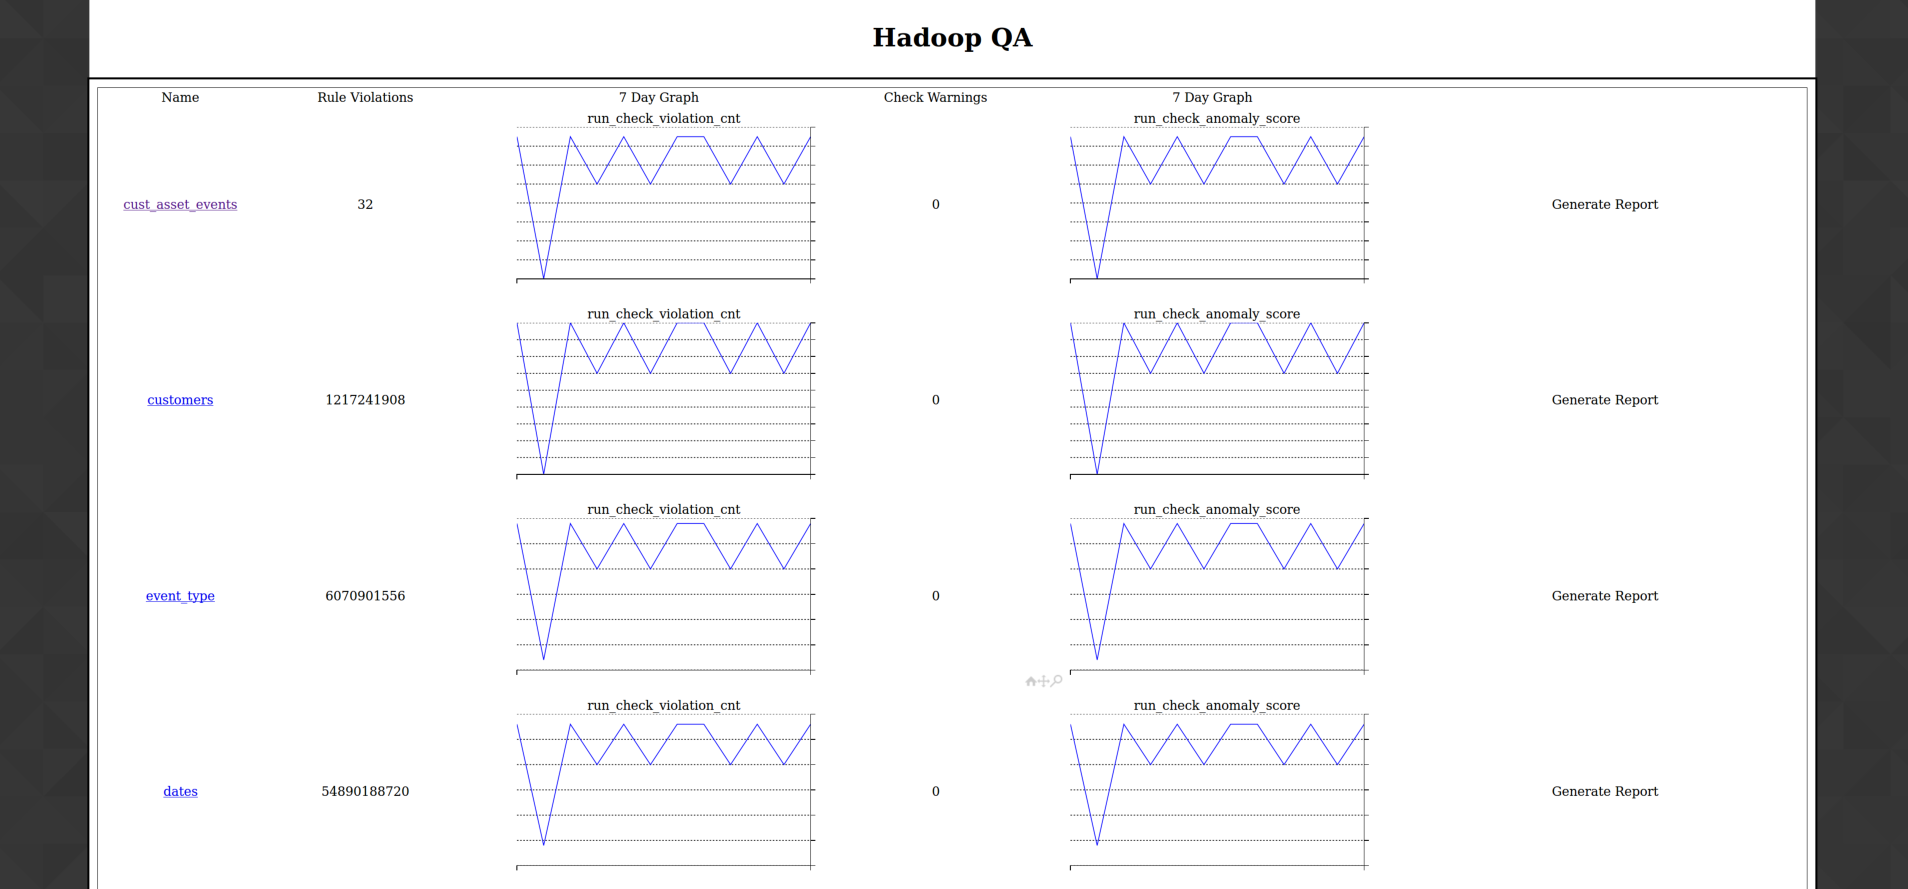
\includegraphics[scale=0.2]{./img/westwind.png}
    \caption{Database View}
\end{figure}
